Convolution of an input with with a linear filter in the termporal or
spatial domain is equivalent to multiplication by the fourier
transforms of the input and the filter in the spectral domain.  This
provides a conceptually simple way to think about filtering: transform
your signal into the frequency domain, dampen the frequencies you are
not interested in by multiplying the frequency spectrum by the desired
weights, and then inverse transform the multiplies spectrum back into
the original domain.  In the example below, we will simply set the
weights of the frequencies we are uninterested in (the high frequency
noise) to zero rather than dampening them with a smoothly varying
function.  Although this is not usually the best thing to do, since
sharp edges in one domain usually introduce artifacts in another (eg
high frequency ``ringing''), it is easy to do and sometimes provides
satisfactory results.

The image in the upper left panel of Figure~\ref{fig:fft_imdenoise} is
a grayscale photo of the moon landing.  There is a banded pattern of
high frequency noise polluting the image.  In the upper right panel we
see the 2D spatial frequency spectrum.  The FFT output in
\texttt{scipy} is packed with the lower freqeuencies starting in the
upper left, and proceeding to higher frequencies as one moves to the
center of the spectrum (this is the most efficient way numerically to
fill the output of the FFT algorithm).  Because the input signal is
real, the output spectrum is complex and symmetrical: the
transformation values beyond the midpoint of the frequency spectrum
(the Nyquist frequency) correspond to the values for negative
frequencies and are simply the mirror image of the positive
frequencies below the Nyquist (this is true for the 1D, 2D and ND FFTs
in \texttt{numpy}).

In this exercise we will compute the 2D spatial frequency spectra of
the luminance image, zero out the high frequency components, and
inverse transform back into the time domain.  We can plot the input
and output images with the \texttt{pylab.imshow} function, but the
images must first be scaled to be withing the 0..1 luminance range.
For best results, it helps to \textit{amplify} the image by some scale
factor, and then \textit{clip} it to set all values greater than one
to one.  This serves to enhance contrast among the darker elements of
the image, so it is not completely dominated by the brighter segments

\lstinputlisting[label=code:fft_imdenoise_skel,caption={IGNORED}]{skel/fft_imdenoise_skel.py}

\begin{figure}
\begin{centering}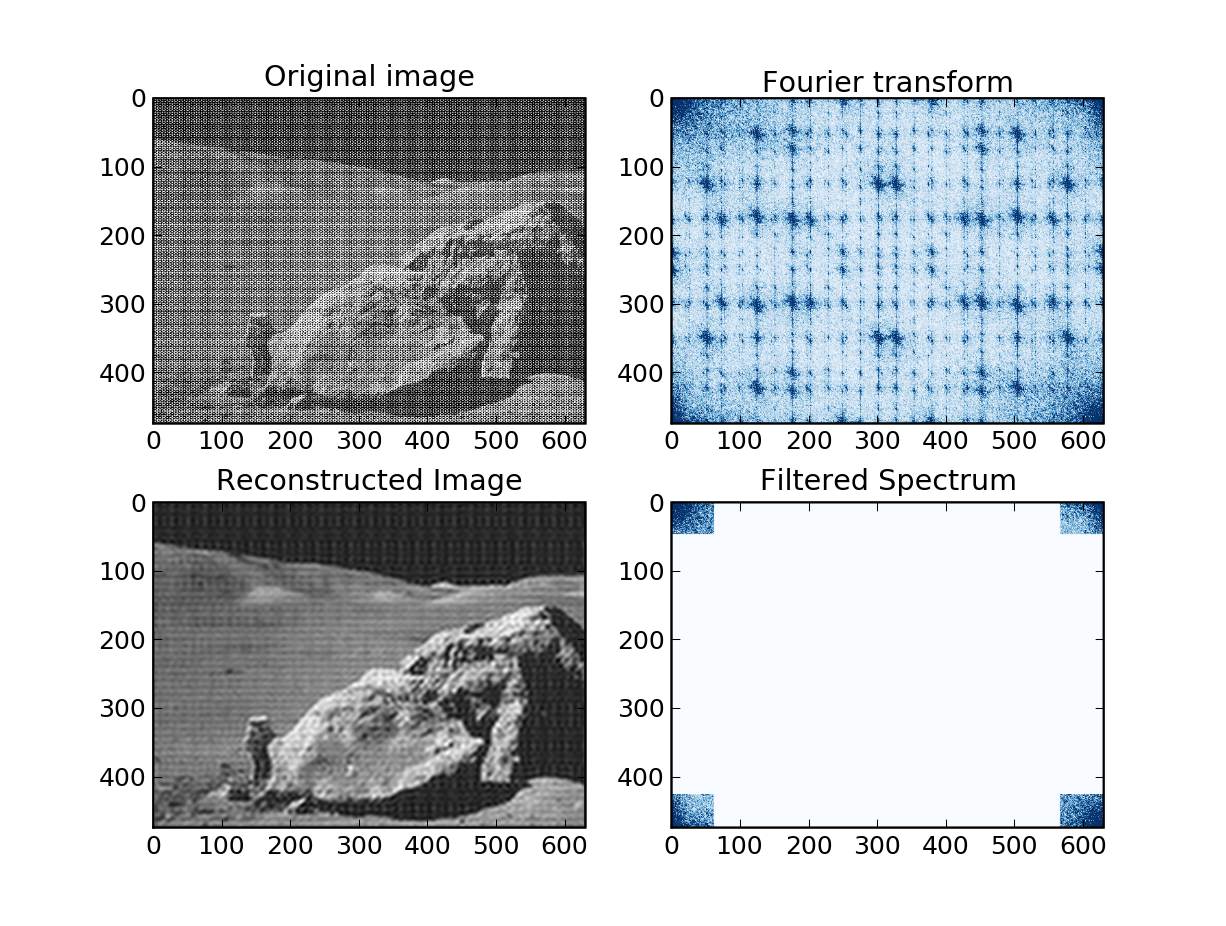
\includegraphics[width=3in]{fig/fft_imdenoise}\par\end{centering}

\caption{\label{fig:fft_imdenoise}High freqeuency noise filtering of a 2D image in the Fourier domain.  The upper panels show the original image (left) and spectral power (right) and the lower panels show the same data with the high frequency power set to zero.  Although the input and output images are grayscale, you can provide colormaps to \texttt{pylab.imshow} to plot them in psudo-color}
\end{figure}
